\chapter{Manual de usuario}
Este manual describirá brevemente el uso del sistema \textbf{BiblioIR: Bibliometry search engine}.

\section{General}
Dicho sistema disponible como web cuenta con dos módulos, la \textbf{búsqueda de autores }(\textit{Author Search}) y la de \textbf{artículos} (\textit{Abstract Search}).

En la siguiente imagen podemos apreciar los componentes principales de la interfaz:
\begin{itemize}
	\item En la parte superior junto al nombre de la aplicación se encuentra la \textbf{barra de búsqueda} donde se introducirán las peticiones.
	\item En la parte inferior e encuentra el \textbf{selector de módulo}, dos pestañas donde podemos elegir entre la búsqueda de autores o artículos. Para saber en cual nos encontramos basta con observar la que se encuentre destacada. Por ejemplo en la imagen se encuentra seleccionada la búsqueda de autores.
\end{itemize}

\begin{figure}[h]
	
	\centering
	
\includegraphics[width=\linewidth]{imagenes/UIcompPrinc}
	\caption{Componentes principales de la interfaz de usuario}
\end{figure}

\section{Búsqueda de autores}
Este módulo de la aplicación permite realizar la búsqueda de los autores de la \myFacultyShort mostrando una tabla con los resultados. Esa tabla muestra el nombre del autor, sus citas totales y su índice h total (tomados del ranking UGRinvetiga) También se muestra unos pequeños metadatos sobre la consulta con el número de resultados y el tiempo que ha llevado al servidor de búsqueda recuperarlos.

\begin{figure}[h]
	
	\centering
	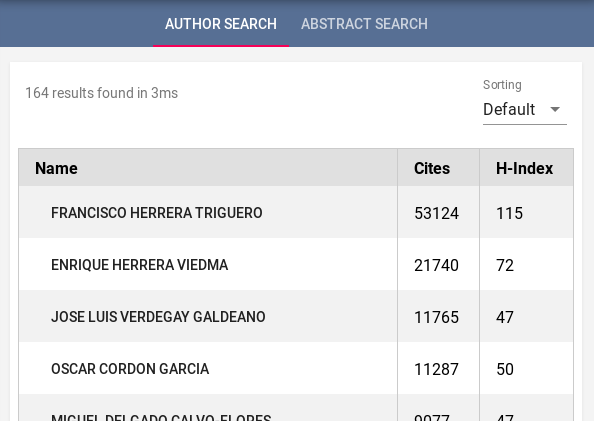
\includegraphics[width=\linewidth]{imagenes/UIAuthor}
	\caption{Búsqueda de autores}
\end{figure}



\newpage
A la derecha de la vista de autores, nos encontramos un menú de selección de ordenamiento que dispone de las opciones que pueden verse en la imagen siguiente y han sido aclaradas en el apartado de desarrollo.


\begin{figure}[h]

	\centering
	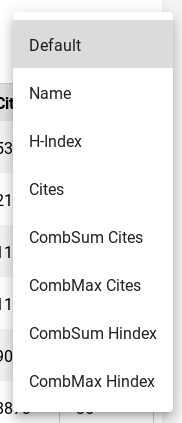
\includegraphics[width=0.20\linewidth]{imagenes/UIAuthorSelection}
	\caption{Ordenación de autores}

\end{figure}


Al seleccionar un autor haciendo click en su nombre se despliega un diálogo donde se nos muestra sus detalles, como se puede ver a continuación. Dicho diálogo contiene botones para acceder a otros perfiles del autor.
\begin{figure}[h]
		  %\vspace{-5pt}
	\centering
	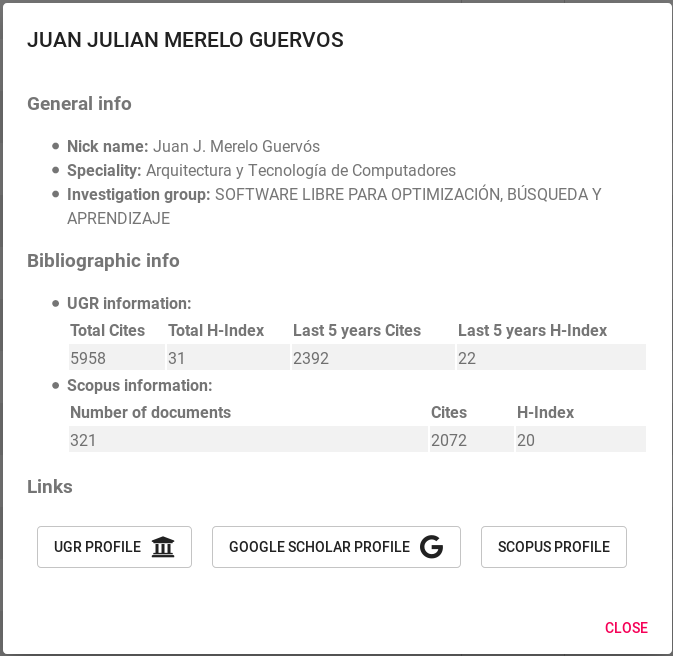
\includegraphics[width=0.7\linewidth]{imagenes/UIAuthorDetail}
	\caption{Vista en detalle de un autor}
	  \vspace{-30pt}
\end{figure}

\section{Búsqueda de artículos}
Este otro módulo, que permite la búsqueda de artículos, cuenta con una interfaz similar, salvo que en lugar de una tabla nos encontramos una lista. Cada elemento representa un artículo y muestra su título, autores, fecha de publicación, número de citas en Scopus y palabras clave si están disponibles.

Cabe destacar que mientras que en la búsqueda de autores se realiza la búsqueda mientras se va escribiendo la petición en el cuadro de búsqueda, en los artículos debido a su mayor número y tamaño es necesario pulsar \texttt{Enter} para lanzar la consulta.
\begin{figure}[h]
	
	\centering
	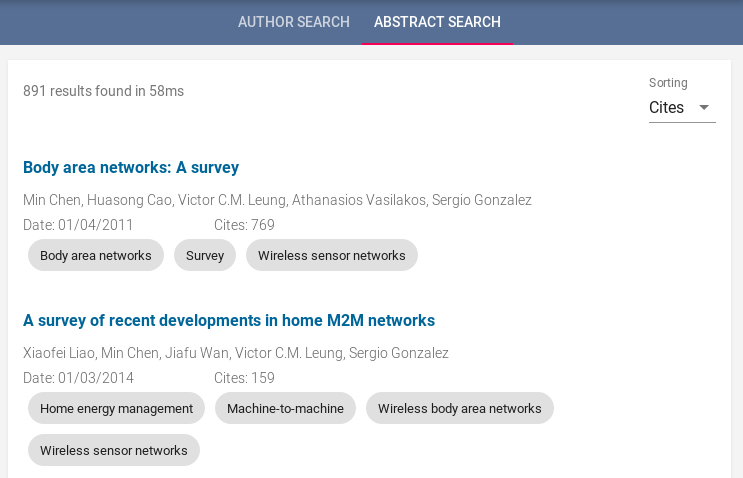
\includegraphics[width=\linewidth]{imagenes/UIAbstract}
	\caption{Búsqueda de artículos}
\end{figure}

\newpage
Al igual que en los autores también disponemos de un menú de selección de ordenación muy similar y con las opciones descritas en desarrollo.

\begin{figure}[h]
	
	\centering
	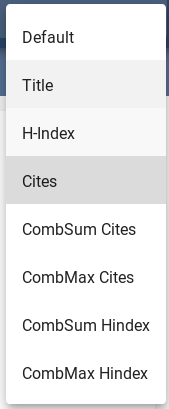
\includegraphics[width=0.20\linewidth]{imagenes/UIAbstractSelection}
	\caption{Ordenación de artículos}
	
\end{figure}

\newpage
Seleccionando alguno de los artículos pasamos a la vista detallada de los mismos, donde vemos una ficha con más datos, un desplegable que muestra el resumen del mismo, un botón para abrirlo en Scopus y las referencias del mismo a otros artículos de la colección (en caso de existir alguna).

\begin{figure}[h]
	%\vspace{-5pt}
	\centering
	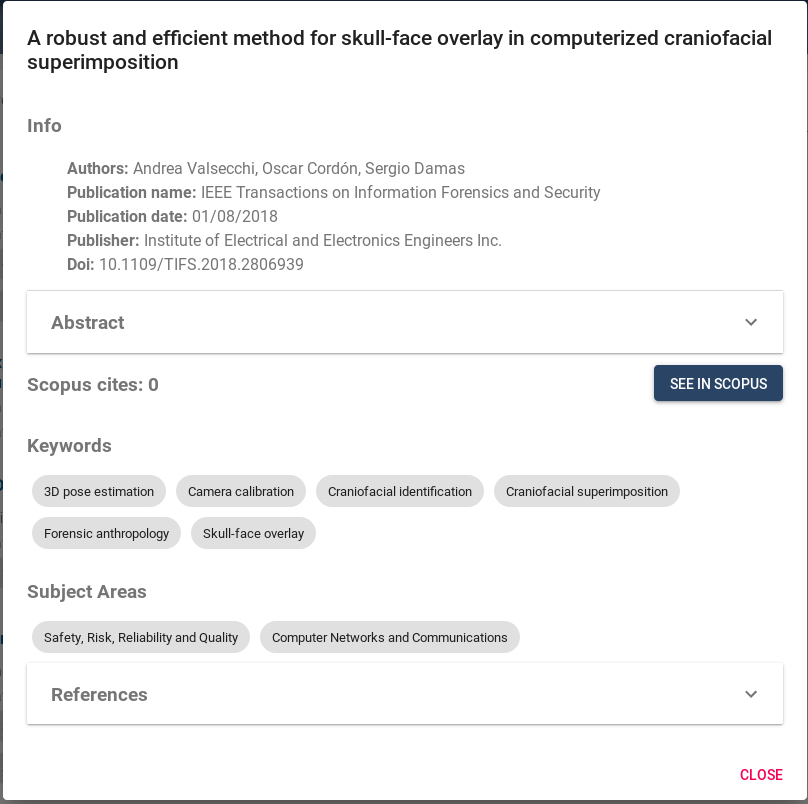
\includegraphics[width=\linewidth]{imagenes/UIAbstractDetail}
	\caption{Vista en detalle de un artículo}
	\vspace{-30pt}
\end{figure}